\begin{answer}{rolltwodice}
The easiest thing to do here is to draw the matrix of possibilities.
(You don't actually have to fill in all the values like in the illustration, drawing a $6 \times 6$ block should be enough to figure out the answer.)
%
\begin{center}
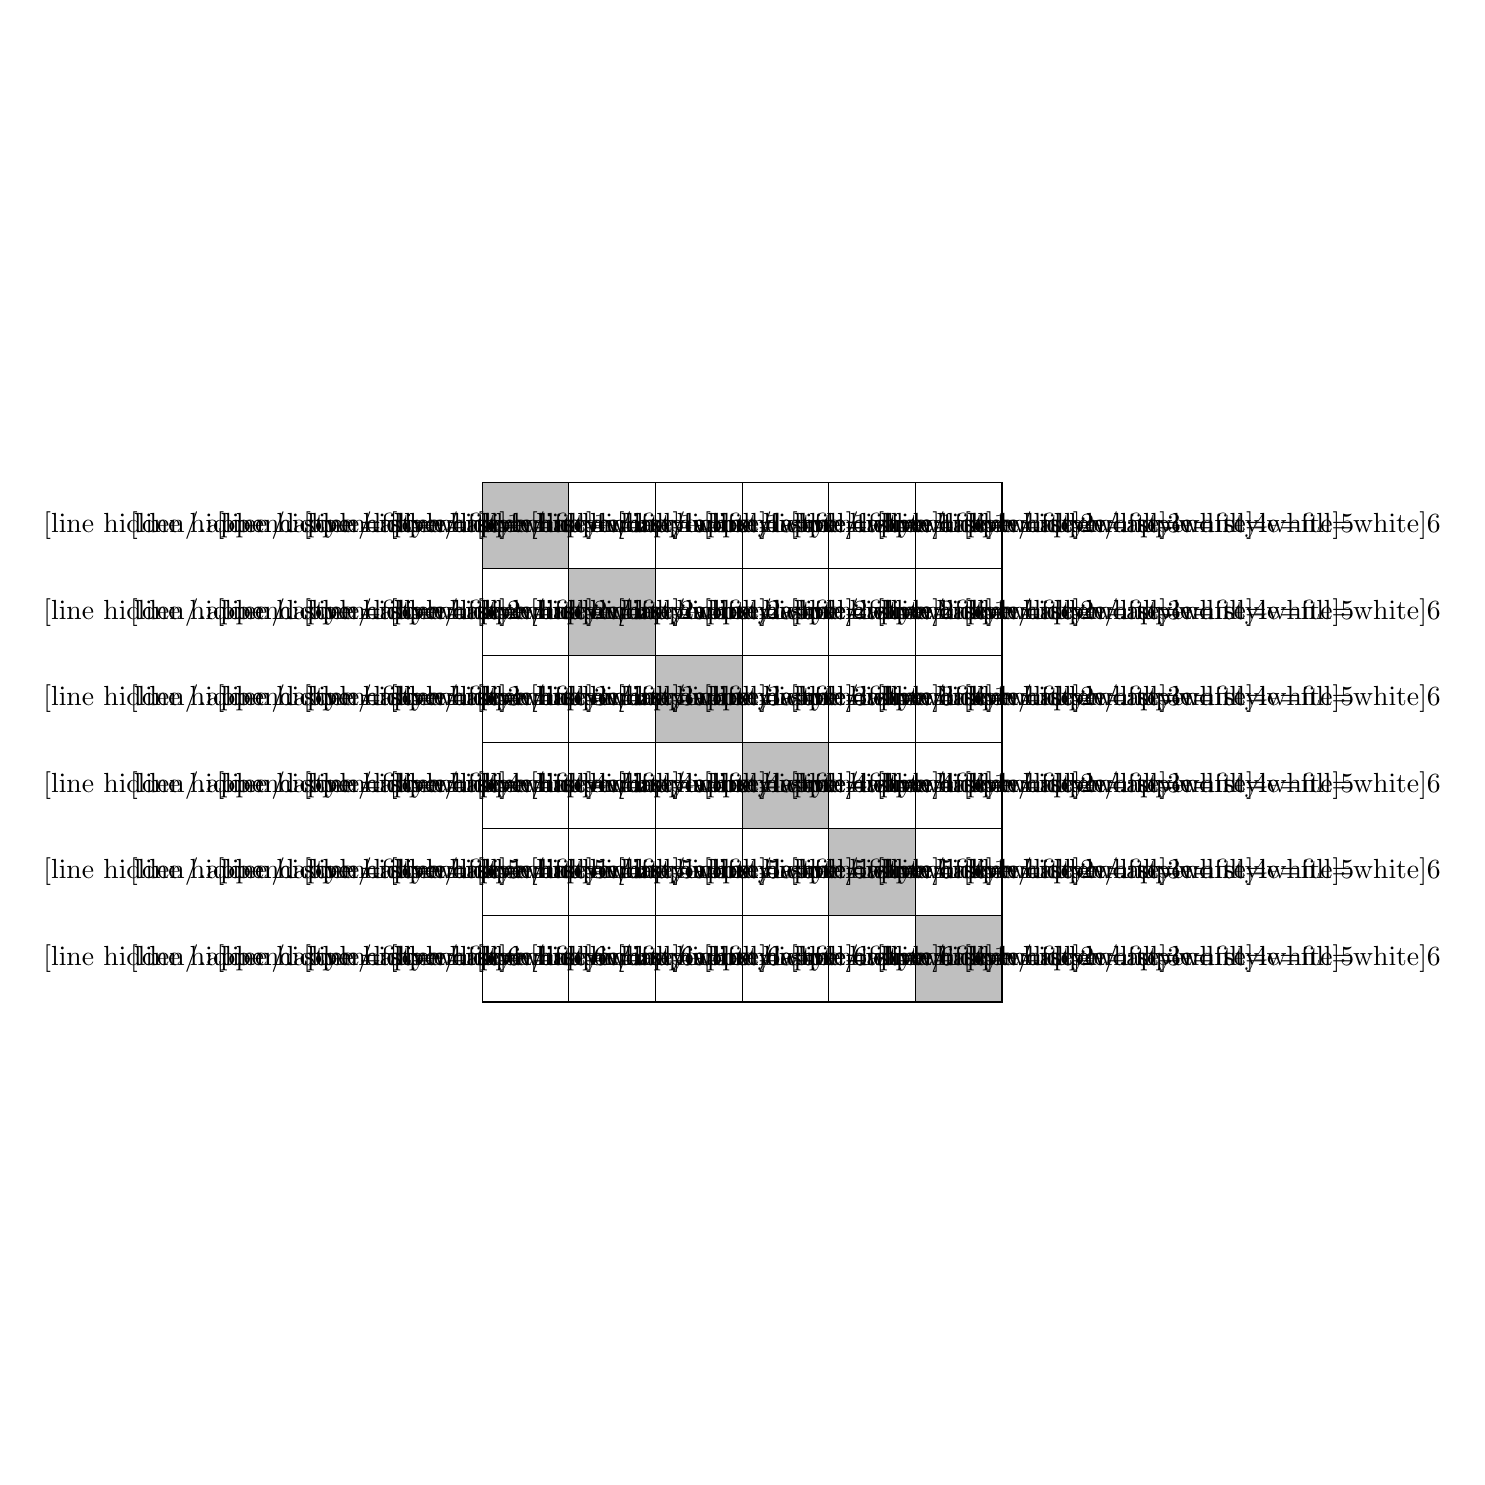
\begin{tikzpicture}[scale=1.1]
% Draw the diagonal (must do this first
\foreach \x in {1,...,6}
{
    % Make the node a circle for space reasons, but don't draw it
    \filldraw[fill=lightgray] (\x,-\x) +(-.5,-.5) rectangle ++(.5,.5);
}
% Draw the matrix
\foreach \x in {1,...,6}
{
  % Make nodes on the outside of the matrix on the right side
  % Label them with o1, o2, etc.
  \foreach \y in {1,...,6}
  {
    \draw (\x,-\y) +(-.5,-.5) rectangle ++(.5,.5);
    % Make the node a circle for space reasons, but don't draw it
    \draw (\x,-\y) node[circle, inner sep=2mm] (n\y\x) {
                                           \drawdie[line hidden/.append style={fill=white}]{\y}
                                           \drawdie[line hidden/.append style={fill=white}]{\x}
                                           }; %reverse the x and y to give the expected behaviour
  }
}
\end{tikzpicture}
\end{center}
%
Now, depending on what the interviewer meant by the question, the answer is one of the following.
\begin{enumerate}
  \item
The probability of one die being larger than the other (not caring which one) is like saying what is the probability that they are not the same.
That is everything but the diagonal,
\[
  \frac{36- 6}{36} =  \frac{30}{36} = \frac{5}{6}
  \text{.}
\]
  \item
If the interviewer wanted the probability of die $A$ being more than die $B$ then the possibilities are everything in the upper/lower triangle of the matrix (half of the answer given above),
\[
  \frac{15}{36} = \frac{5}{12}
  \text{.}
\]
\end{enumerate}

This is a great question to start with, as it shows a trick often employed by these brainteasers.
When presented with a questions like this, one might be inclined to start writing out the calculations (involving tedious sums or integrals).
However, many of these types of questions can be quickly solved by drawing a square on which you can calculate the area without doing integrals.
Other examples are the
\emph{Stick Breaking} problem (question \ref{q:stickbreak})
and
\emph{Romeo and Juliet} (question \ref{q:romeojuliet}),
which we will encounter later.

This simple example shows the importance of interview preparation.
One might think that, on the job, a rigorous solution is preferred to a back-of-the-envelope one.
One might be right, but the interviews aren't testing for job preparedness.
They are probably trying to test for several qualities, but they end up selecting the candidates who are the most prepared for brainteasers.
The format is akin to asking candidates to do a Rubik's cube and preferring the one who memorised the solution by rote and solves it in two minutes, rather than the one who takes the cube home and solves it over the course of three months without looking at the solution online.
Who would you rather have work for you?
Your answer is irrelevant.
Just know that brainteasers favour the former candidate and keep it in mind during preparation.
Use the pretty solution during the interview and leave the rigorous integrals for a Saturday night with a glass of whiskey in your study, while reflecting on the fact that people in quantitative finance are probably all brainteaser savants.
\end{answer}
